\documentclass[journal,12pt,twocolumn]{IEEEtran}

\usepackage{setspace}
\usepackage{gensymb}

\singlespacing


\usepackage[cmex10]{amsmath}

\usepackage{amsthm}

\usepackage{mathrsfs}
\usepackage{txfonts}
\usepackage{stfloats}
\usepackage{bm}
\usepackage{cite}
\usepackage{cases}
\usepackage{subfig}

\usepackage{longtable}
\usepackage{multirow}

\usepackage{enumitem}
\usepackage{mathtools}
\usepackage{steinmetz}
\usepackage{tikz}
\usepackage{circuitikz}
\usepackage{verbatim}
\usepackage{tfrupee}
\usepackage[breaklinks=true]{hyperref}
\usepackage{graphicx}
\usepackage{tkz-euclide}
\usepackage{float}

\usetikzlibrary{calc,math}
\usepackage{listings}
    \usepackage{color}                                            %%
    \usepackage{array}                                            %%
    \usepackage{longtable}                                        %%
    \usepackage{calc}                                             %%
    \usepackage{multirow}                                         %%
    \usepackage{hhline}                                           %%
    \usepackage{ifthen}                                           %%
    \usepackage{lscape}     
\usepackage{multicol}
\usepackage{chngcntr}

\DeclareMathOperator*{\Res}{Res}

\renewcommand\thesection{\arabic{section}}
\renewcommand\thesubsection{\thesection.\arabic{subsection}}
\renewcommand\thesubsubsection{\thesubsection.\arabic{subsubsection}}

\renewcommand\thesectiondis{\arabic{section}}
\renewcommand\thesubsectiondis{\thesectiondis.\arabic{subsection}}
\renewcommand\thesubsubsectiondis{\thesubsectiondis.\arabic{subsubsection}}


\hyphenation{op-tical net-works semi-conduc-tor}
\def\inputGnumericTable{}                                 %%

\lstset{
%language=C,
frame=single, 
breaklines=true,
columns=fullflexible
}
\begin{document}


\newtheorem{theorem}{Theorem}[section]
\newtheorem{problem}{Problem}
\newtheorem{proposition}{Proposition}[section]
\newtheorem{lemma}{Lemma}[section]
\newtheorem{corollary}[theorem]{Corollary}
\newtheorem{example}{Example}[section]
\newtheorem{definition}[problem]{Definition}

\newcommand{\BEQA}{\begin{eqnarray}}
\newcommand{\EEQA}{\end{eqnarray}}
\newcommand{\define}{\stackrel{\triangle}{=}}
\bibliographystyle{IEEEtran}
\providecommand{\mbf}{\mathbf}
\providecommand{\pr}[1]{\ensuremath{\Pr\left(#1\right)}}
\providecommand{\qfunc}[1]{\ensuremath{Q\left(#1\right)}}
\providecommand{\sbrak}[1]{\ensuremath{{}\left[#1\right]}}
\providecommand{\lsbrak}[1]{\ensuremath{{}\left[#1\right.}}
\providecommand{\rsbrak}[1]{\ensuremath{{}\left.#1\right]}}
\providecommand{\brak}[1]{\ensuremath{\left(#1\right)}}
\providecommand{\lbrak}[1]{\ensuremath{\left(#1\right.}}
\providecommand{\rbrak}[1]{\ensuremath{\left.#1\right)}}
\providecommand{\cbrak}[1]{\ensuremath{\left\{#1\right\}}}
\providecommand{\lcbrak}[1]{\ensuremath{\left\{#1\right.}}
\providecommand{\rcbrak}[1]{\ensuremath{\left.#1\right\}}}
\theoremstyle{remark}
\newtheorem{rem}{Remark}
\newcommand{\sgn}{\mathop{\mathrm{sgn}}}
\providecommand{\abs}[1]{\lvert#1\vert}
\providecommand{\res}[1]{\Res\displaylimits_{#1}} 
\providecommand{\norm}[1]{\lVert#1\rVert}
%\providecommand{\norm}[1]{\lVert#1\rVert}
\providecommand{\mtx}[1]{\mathbf{#1}}
\providecommand{\mean}[1]{E[ #1 ]}
\providecommand{\fourier}{\overset{\mathcal{F}}{ \rightleftharpoons}}
%\providecommand{\hilbert}{\overset{\mathcal{H}}{ \rightleftharpoons}}
\providecommand{\system}{\overset{\mathcal{H}}{ \longleftrightarrow}}
	%\newcommand{\solution}[2]{\textbf{Solution:}{#1}}
\newcommand{\solution}{\noindent \textbf{Solution: }}
\newcommand{\cosec}{\,\text{cosec}\,}
\providecommand{\dec}[2]{\ensuremath{\overset{#1}{\underset{#2}{\gtrless}}}}
\newcommand{\myvec}[1]{\ensuremath{\begin{pmatrix}#1\end{pmatrix}}}
\newcommand{\mydet}[1]{\ensuremath{\begin{vmatrix}#1\end{vmatrix}}}
\numberwithin{equation}{subsection}
\makeatletter
\@addtoreset{figure}{problem}
\makeatother
\let\StandardTheFigure\thefigure
\let\vec\mathbf
\renewcommand{\thefigure}{\theproblem}
\def\putbox#1#2#3{\makebox[0in][l]{\makebox[#1][l]{}\raisebox{\baselineskip}[0in][0in]{\raisebox{#2}[0in][0in]{#3}}}}
     \def\rightbox#1{\makebox[0in][r]{#1}}
     \def\centbox#1{\makebox[0in]{#1}}
     \def\topbox#1{\raisebox{-\baselineskip}[0in][0in]{#1}}
     \def\midbox#1{\raisebox{-0.5\baselineskip}[0in][0in]{#1}}
\vspace{3cm}
\title{Assignment-4}
\author{UNNATI GUPTA}
\maketitle
\newpage
\bigskip
\renewcommand{\thefigure}{\theenumi}
\renewcommand{\thetable}{\theenumi}
Download all python codes from 
\begin{lstlisting}
https://github.com/unnatigupta2320/Assignment_4/tree/master/codes
\end{lstlisting}
%
and latex-tikz codes from 
%
\begin{lstlisting}
https://github.com/unnatigupta2320/Assignment_4
\end{lstlisting}
%
\section{Question No. 2.17}
Find the perpendicular distance of the following lines from the origin and angle between the perpendicular and positive x-axis.
\begin{enumerate}[label=\alph*.]
    \item  $\myvec{1&-\sqrt{3}}\vec{x} =-8$
    \item  $\myvec{0&1}\vec{x} =2$
    \item $\myvec{1&-1}\vec{x} =4$
\end{enumerate}
%
\section{Solution}
\begin{enumerate}
\item  All the given data can be tabularised in table \ref{tab:table1}:
\numberwithin{table}{section}
\begin{table}[!ht]
\begin{center}
\begin{tabular}{ | m{2cm} | m{1.2cm}| m{1.2cm} | m{1.2cm} |} 
\hline
 & Line\textsubscript{1} & Line\textsubscript{2} & Line\textsubscript{3} \\
\hline
c\textsubscript{1},c\textsubscript{2},c\textsubscript{3} & 8 & -2 & -4 \\ 
\hline
$\vec{n\textsubscript{1}}$,$\vec{n\textsubscript{2}}$,$\vec{n\textsubscript{3}}$ & $\myvec{1\\-\sqrt{3}}$ & $\myvec{0\\1}$ &$\myvec{1\\-1}$ \\ 
\hline
\end{tabular}
\end{center}
\caption{Given Data}
\label{tab:table1}
\end{table}
\item For finding the perpendicular distance of lines from origin:-
\begin{itemize}
\item The formula for calculating perpendicular distance between the point and a given line is :
\begin{align}
d=\frac { \left| c-\vec{n}^T\vec{A} \right| }{ \norm{\vec{n}} }
\end{align}
where,$\vec{n}$ is the normal vector of line.
\item If we have to find distance from origin, then above formula get reduced to:
\begin{align}
d&=\frac { \left| c \right| }{\norm{\vec{n}}}\label{eqA}
\end{align}
\end{itemize}
\item For finding angle between the perpendicular and positive x-axis:-
\begin{itemize}
\item If e\textsubscript{1}=$\myvec{1\\0}$ is the direction vector of x-axis then the angle $\theta$  between line and x-axis,is given using inner products of vectors as:
\begin{align}
\cos \theta&=\frac{\vec{n}^T\vec{e\textsubscript{1}}}{\norm{\vec{n}}\times\norm{\vec{e\textsubscript{1}}}}
  \\
 \implies \theta &= \cos^{-1}\frac{\vec{n}^T\vec{e\textsubscript{1}}}{\norm{\vec{n}}\times\norm{\vec{e\textsubscript{1}}}}\label{eqD}
\end{align}
\end{itemize}
\begin{enumerate}[label=\alph*.]
\item $Line_1$, $\myvec{1&-\sqrt{3}}\vec{x}$ =$-8$
\begin{itemize}
\item We have:
\begin{align}
 c\textsubscript{1}=8 , {\vec{n\textsubscript{1}}}=\myvec{1\\-\sqrt{3}}  
\end{align}
\item Using \eqref{eqA} we get:
\begin{align}
d&=\frac { \left| c\textsubscript{1} \right| }{\norm{\vec{n\textsubscript{1}}}}
\\
d&=\frac{8}{\sqrt{1+3}} 
\\
d&=\frac{8}{2}=4\text{ units}
\end{align}
\item The direction vector $\vec{n}$ of the line perpendicular to given line is: 
\begin{align}
    \vec{n}=\myvec{-1\\\sqrt{3}}
\end{align}
\item Using \eqref{eqD} the angle which perpendicular is making with positive x-axis is:
\begin{align}
   \cos\theta &= \frac{\vec{n}^T\vec{e\textsubscript{1}}}{\norm{\vec{n}}\times\norm{\vec{e\textsubscript{1}}}}
   \\
   \cos\theta&= \frac{\myvec{-1&\sqrt{3}}\myvec{1\\0}}{\sqrt{4}\times\sqrt{1}}
     \\
 \cos\theta &= \frac{-1}{2}
 \\
 \implies \theta&=\cos^{-1}(-0.5)
 \\
 \therefore  \theta&=120\degree
\end{align}
\end{itemize}
\item $Line_2$, $\myvec{0&1}\vec{x} =2$
\begin{itemize}
\item We have:
\begin{align}
 c\textsubscript{2}=-2 ,{\vec{n\textsubscript{2}}}=\myvec{0\\1}   
\end{align}
\item Using \eqref{eqA} we get:
\begin{align}
d&=\frac { \left| c\textsubscript{2} \right| }{\norm{\vec{n\textsubscript{2}}}}
\\
d&=\frac{2}{\sqrt{1}} 
\\
d&=2 \text{ units}
\end{align}
\item The direction vector $\vec{n}$ of the line perpendicular to given line is: 
\begin{align}
    \vec{n}=\myvec{0\\1}
\end{align}
\item Using \eqref{eqD} the angle which perpendicular is making with positive x-axis is:
\begin{align}
   \cos\theta &= \frac{\vec{n}^T\vec{e\textsubscript{1}}}{\norm{\vec{n}}\times\norm{\vec{e\textsubscript{1}}}}
    \end{align}
    \begin{align}
   \cos\theta &= \frac{\myvec{0&1}\myvec{1\\0}}{\sqrt{1}\times\sqrt{1}}
    \\
 \cos\theta&= 0
 \\
 \implies \theta&=\cos^{-1}(0)
 \\
 \therefore  \theta&=90\degree
\end{align}
\end{itemize}
\item 
$Line_3$,$\myvec{1&-1}\vec{x} =4$
\begin{itemize}
\item We have:
\begin{align}
 c\textsubscript{3}= -4 ,{\vec{n\textsubscript{3}}}=\myvec{1\\-1}   
\end{align}
\item Using \eqref{eqA} we get:
\begin{align}
d&=\frac { \left| c\textsubscript{3}\right| }{\norm{\vec{n\textsubscript{3}}}}
\\
d&=\frac{4}{\sqrt{1+1}} 
\\
d&=\frac{4}{\sqrt{2}}
\\
d&=\frac{4}{1.41}
\\
d&=2.828 \text{ units}
\end{align}
\item The direction vector $\vec{n}$ of the line perpendicular to given line is: 
\begin{align}
    \vec{n}=\myvec{-1\\1}
\end{align}
\item Using \eqref{eqD} the angle which perpendicular is making with positive x-axis is:
\begin{align}
   \cos\theta&= \frac{\vec{n}^T\vec{e\textsubscript{1}}}{\norm{\vec{n}}\times\norm{\vec{e\textsubscript{1}}}}
    \end{align}
    \begin{align}
   \cos\theta &= \frac{\myvec{-1&1}\myvec{1\\0}}{\sqrt{2}\times\sqrt{1}}
    \\
 \cos\theta&= \frac{-1}{\sqrt{2}}
 \\
 \implies \theta&=\cos^{-1}\frac{-1}{\sqrt{2}}
 \\
 \therefore  \theta&=135\degree
\end{align}
\end{itemize}
\end{enumerate}
\item If,
\\
\textbf{d\textsubscript{n}}=Perpendicular distance of line from origin
\\
\\
$\theta\textsubscript{n}$= Angle of perpendicular with positive x-axis.
\item All the calculated data can be tabularised in table  \ref{tab:table2}:
\end{enumerate}
\numberwithin{table}{section}
\begin{table}[!ht]
\begin{center}
\begin{tabular}{ | m{2cm} | m{1.2cm}| m{1.2cm} | m{1.2cm} |} 
\hline
 & Line\textsubscript{1} & Line\textsubscript{2} & Line\textsubscript{2} \\
\hline
d\textsubscript{1},d\textsubscript{2},d\textsubscript{3} & 4 & 2 & 2.828 \\ 
\hline
$\theta\textsubscript{1}$,$\theta\textsubscript{2}$,$\theta\textsubscript{3}$& $120\degree$ & $90\degree$ & $135\degree$ \\ 
\hline
\end{tabular}
\end{center}
\caption{Calculated Data}
\label{tab:table2}
\end{table}
\begin{itemize}
\item The plots of all the three lines and there respective perpendiculars are as follows:-
\end{itemize}
\numberwithin{figure}{section}
\begin{figure}[H]
\centering
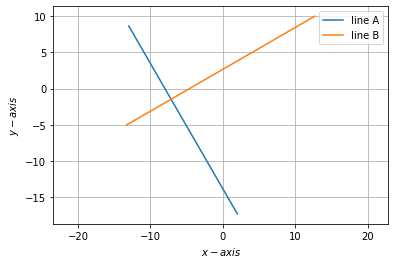
\includegraphics[width=\columnwidth]{Line1 and it's perpendicular.png}
\caption{Line\textsubscript{1} and it's perpendicular}
\label{fig:circle}	
\end{figure}
\numberwithin{figure}{section}
\begin{figure}[H]
\centering
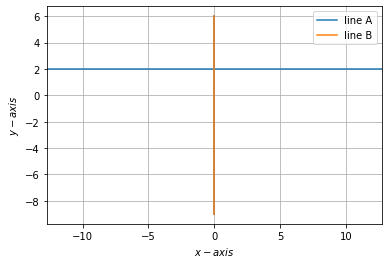
\includegraphics[width=\columnwidth]{Line2 and it's perpendicular.png}
\caption{Line\textsubscript{2} and it's perpendicular}
\label{fig:circle}	
\end{figure}
\numberwithin{figure}{section}
\begin{figure}[H]
\centering
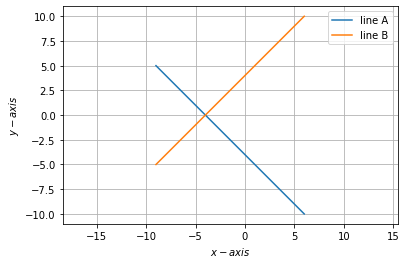
\includegraphics[width=\columnwidth]{Line3 and it's perpendicular.png}
\caption{Line\textsubscript{3} and it's perpendicular}
\label{fig:circle}	
\end{figure}
\end{document}